\documentclass[12pt,a4paper,openright]{book}

% === Pacotes ===
\usepackage[utf8]{inputenc}
\usepackage[T1]{fontenc}
\usepackage[portuguese]{babel}
\usepackage{geometry}
\usepackage{graphicx}
\usepackage{xcolor}
\usepackage{hyperref}
\usepackage{setspace}
\usepackage{titlesec}
\usepackage{fancyhdr}
\usepackage{indentfirst}
\usepackage{enumitem}
\usepackage{bookmark}
\usepackage{epigraph}

% === Geometria ===
\geometry{top=3cm, bottom=2.5cm, left=3cm, right=2.5cm}

% === Estilo de capítulos ===
\titleformat{\chapter}[display]
  {\normalfont\huge\bfseries\color{red!70!black}}
  {\filleft\MakeUppercase{\chaptertitlename}\hspace{1ex}\Huge\thechapter}
  {20pt}{\Huge\bfseries\filcenter}
\titlespacing*{\chapter}{0pt}{0pt}{40pt}

\titleformat{\section}
  {\normalfont\Large\bfseries\color{red!50!black}}
  {\thesection}{1em}{}

% === Cabeçalho/Rodapé ===
\pagestyle{fancy}
\fancyhf{}
\fancyhead[LE,RO]{\thepage}
\fancyhead[RE]{\leftmark}
\fancyhead[LO]{\rightmark}
\renewcommand{\headrulewidth}{0.5pt}

% === Meta-informação ===
\title{O Grande Livro do Cuscuz}
\author{Uma Viagem pelos Tipos, Sabores e Histórias}
\date{2026}

\begin{document}

% ============================================================
% CAPA
% ============================================================
\begin{titlepage}
\centering
\vspace*{2cm}
{\Huge\bfseries\color{red!70!black} O Grande Livro do Cuscuz}\\[1cm]
{\Large Uma Viagem pelos Tipos, Sabores e Histórias}\\[2cm]
{\large Aleksandro}\\[2cm]
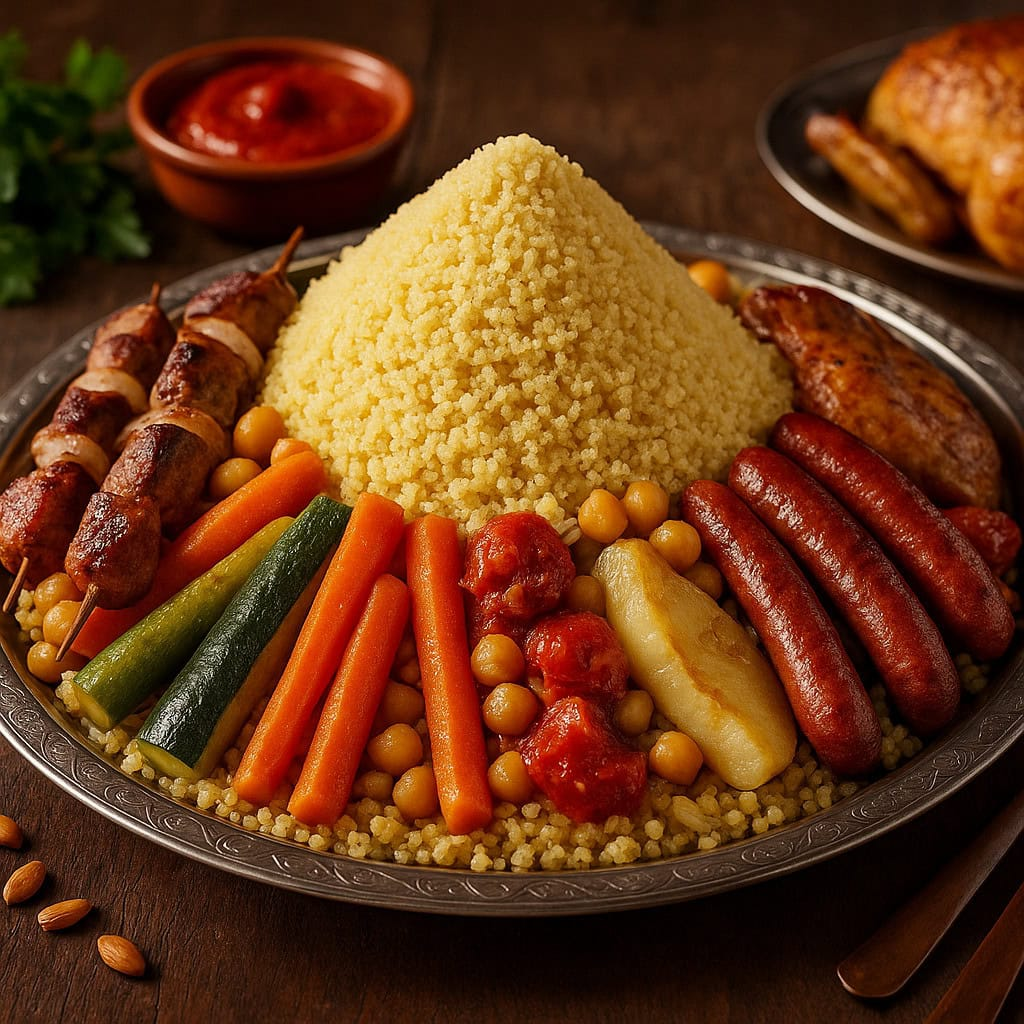
\includegraphics[width=0.7\textwidth]{livro-cuscuz-imagens/cuscuz-marroquino.jpg}\\[1cm]
{\large 2026}
\end{titlepage}

% ============================================================
% FOLHA DE ROSTO
% ============================================================
\newpage
\thispagestyle{empty}
\vspace*{4cm}
\begin{center}
{\Huge\bfseries O Grande Livro do Cuscuz}\\[1cm]
{\large Uma Viagem pelos Tipos, Sabores e Histórias}\\[2cm]
{\large Aleksandro}\\[1cm]
{\large 2026}
\end{center}

% ============================================================
% SUMÁRIO
% ============================================================
\tableofcontents
\newpage

% ============================================================
% INTRODUÇÃO
% ============================================================
\chapter*{Introdução}
\addcontentsline{toc}{chapter}{Introdução}

O cuscuz é muito mais do que um alimento. É um fio condutor que atravessa milénios, continentes e culturas. Das tendas berberes no Norte de África às mesas das famílias nordestinas, dos tabuleiros das quitandeiras paulistas do século XIX aos supermercados de todo o mundo, o cuscuz acompanha a história da humanidade.

Este livro nasce de uma pergunta simples --- \textit{quais os tipos de cuscuz?} --- e se transforma numa viagem pelas suas histórias, origens, ingredientes e modos de preparo. Aqui encontrará desde o cuscuz marroquino mais antigo, passando pelo amado cuscuz nordestino de cada manhã, pelo polémico e festivo cuscuz paulista, até ao doce e cremoso cuscuz de tapioca.

Cada capítulo é dedicado a um tipo de cuscuz, com a sua história, características e modos de preparo. No final, incluímos receitas para que o leitor possa recriar cada um destes tesouros gastronómicos na sua própria cozinha.

Bom apetite e boa viagem!

% ============================================================
% CAPÍTULO 1
% ============================================================
\chapter{As Origens: O Cuscuz no Magrebe}

\epigraph{O cuscuz é o prato do dia em Marrocos e na Argélia, e tem estatuto de prato nacional na Tunísia.}{\textit{Enciclopédia Livre}}

\section{Os Primórdios Berberes}

A história do cuscuz começa há milhares de anos, muito antes de qualquer registo escrito. Acredita-se que o cuscuz tenha surgido entre os povos berberes, habitantes originais do Norte de África, numa região conhecida como Magrebe --- que hoje compreende Marrocos, Argélia, Tunísia, Líbia e Mauritânia.

Os berberes, pastores nómadas e agricultores, desenvolveram uma técnica simples mas genial: triturar grãos de cereal, humedecê-los ligeiramente e enrolá-los à mão até formarem pequenas bolotas, que eram então cozidas no vapor. O resultado era um alimento leve, nutritivo e que se conservava bem --- ideal para as longas travessias pelo deserto.

A palavra \textit{cuscuz} deriva do termo berbere \textit{k'seksu} ou \textit{seksu}, que muitos acreditam ser uma onomatopeia do som do vapor a escapar da panela durante o cozimento. Os franceses, ao colonizarem a Argélia, aportuguesaram a palavra para \textit{couscous}, que acabou por se espalhar pelo mundo ocidental.

\section{O Primeiro Registo Escrito}

Uma das referências mais antigas ao cuscuz aparece num livro de receitas do Alandalus (a Península Ibérica sob domínio muçulmano), intitulado \textit{Kitāb al-ṭabīkh fī al-Maghrib wa'l-Āndalus} (\textit{Livro de Culinária do Magrebe e Andaluzia}), do século XIII. O manuscrito utiliza a palavra \textit{alcuzcuz}, indicando que a preparação já era conhecida e apreciada em ambos os lados do Mediterrâneo.

O historiador Clifford Wright sugere que o cuscuz pode ter origens ainda mais antigas, possivelmente sub-saarianas, apontando para o facto de serem mulheres negras as principais cozinheiras no Norte de África e da Alandalus, e para a popularidade de preparações semelhantes na África Ocidental.

\section{O Cuscuz no Mundo Árabe e no Mediterrâneo}

Com a expansão islâmica, o cuscuz espalhou-se por todo o mundo árabe e mediterrâneo. Em cada lugar, ganhou características próprias:

\begin{itemize}
    \item \textbf{Marrocos:} servido tradicionalmente às sextas-feiras após a oração do meio-dia, com um molho de sete vegetais e frango. A versão doce, com amêndoas, cebola caramelizada e especiarias, é reservada para dias de festa.
    \item \textbf{Tunísia:} considerado prato nacional, frequentemente preparado com carne de borrego e frutas secas. A versão mais famosa usa o estômago do borrego recheado com ervas aromáticas.
    \item \textbf{Argélia:} consumido diariamente, acompanhado por molhos de legumes, peixe, aves ou até carne de camelo.
    \item \textbf{Palestina:} conhecido como \textit{maftoul}, um tipo especial de cuscuz feito à mão, rolado com triguilho e farinha de trigo.
\end{itemize}

Em 2020, a UNESCO reconheceu os conhecimentos e práticas relacionados ao preparo do cuscuz como Património Cultural Imaterial da Humanidade, numa candidatura conjunta de Marrocos, Argélia, Tunísia e Mauritânia.

% ============================================================
% CAPÍTULO 2
% ============================================================
\chapter{O Cuscuz no Brasil: Uma História de Adaptação}

\begin{figure}[htbp]
\centering
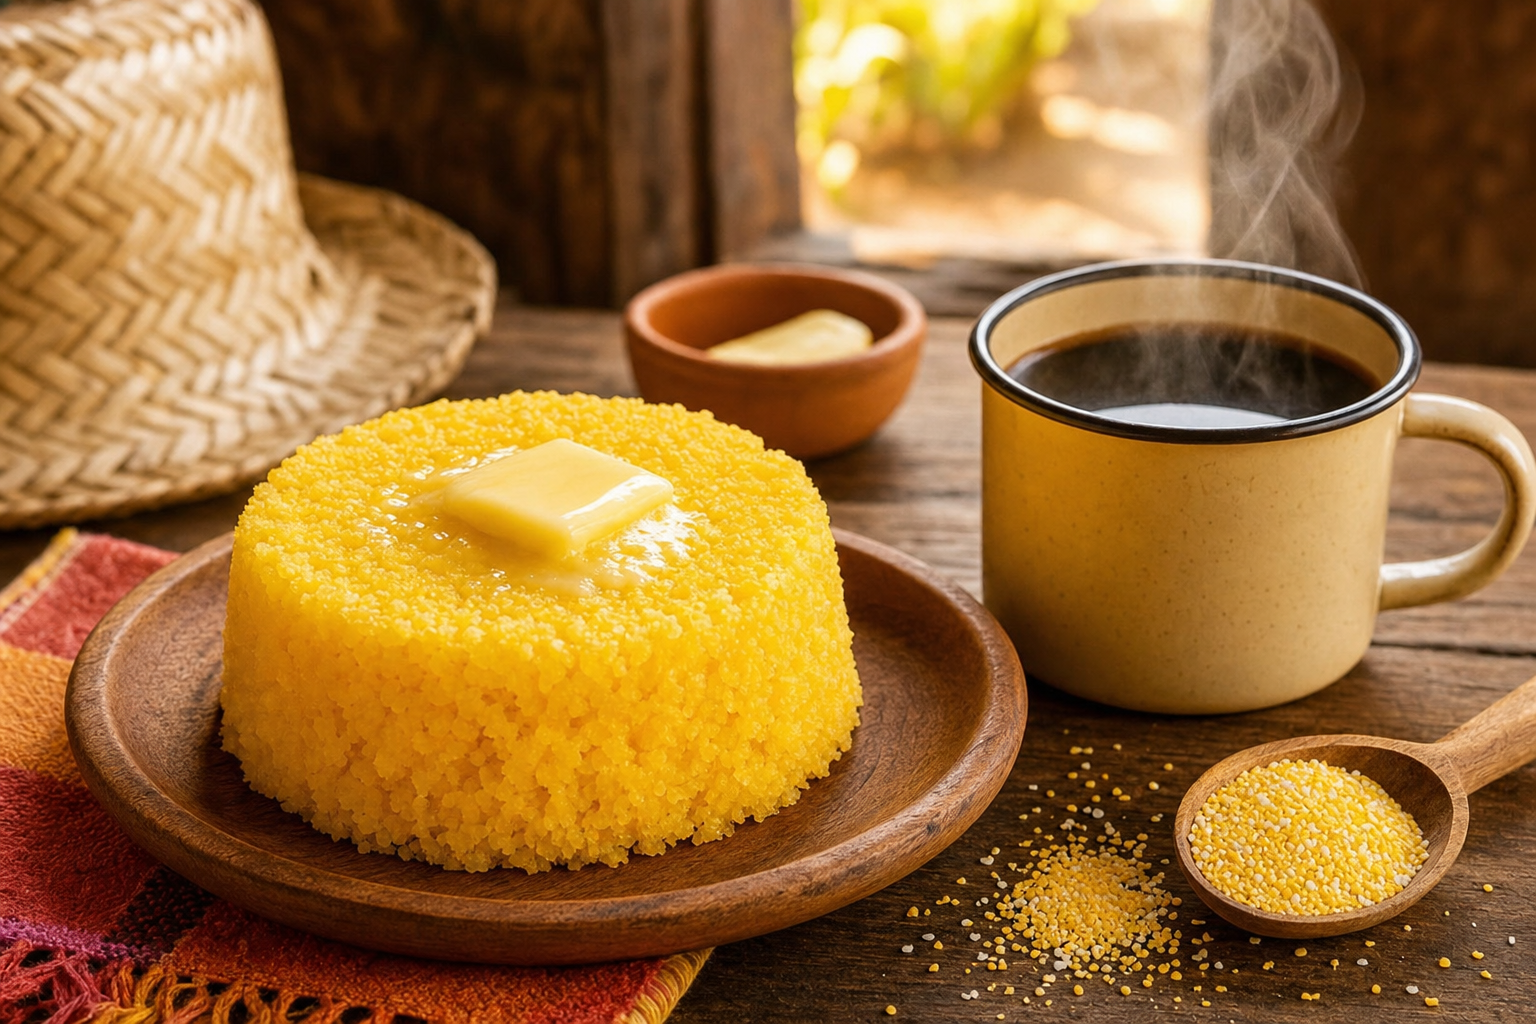
\includegraphics[width=0.85\textwidth]{livro-cuscuz-imagens/cuscuz-nordestino.png}
\caption{Cuscuz nordestino servido com manteiga derretida, o clássico café da manhã do Nordeste brasileiro.}
\label{fig:cuscuz-nordestino}
\end{figure}

\section{A Chegada com os Portugueses}

O cuscuz chegou ao Brasil no século XVI, trazido pelos colonizadores portugueses. Em Portugal, o prato era tão popular que no século XVI fazia parte da ementa diária, sendo mencionado até numa peça de Gil Vicente.

No entanto, a sêmola de trigo usada no cuscuz magrebino era cara e difícil de encontrar no Brasil colónia. Os portugueses e africanos que aqui chegavam encontraram um cereal nativo que já era amplamente cultivado pelos povos indígenas: o milho.

A primeira menção ao cuscuz adaptado ao milho no Brasil data de dezembro de 1585, na Bahia, numa carta do padre José de Anchieta, que relatou que os indígenas \textit{“fazem farinha que fica como cuscuz de farinha de trigo”}.

\section{A Contribuição Indígena e Africana}

Os povos indígenas já dominavam técnicas de processamento do milho, moendo os grãos em pilões para obter farinha. Essa farinha de milho passou a ser usada no lugar da sêmola de trigo, dando origem a uma nova família de cuscuz.

Mas foram as mãos das mulheres africanas escravizadas --- as quitandeiras, cozinheiras e vendedeiras --- que verdadeiramente transformaram o cuscuz brasileiro. Elas experimentaram, adaptaram e criaram variações que se espalharam por todo o território, combinando ingredientes indígenas, europeus e africanos com uma criatividade ímpar.

O escritor e folclorista Luís da Câmara Cascudo, na sua obra \textit{História da Alimentação no Brasil}, documentou como o cuscuz se tornou um alimento transversal a todas as classes sociais, presente tanto nas mesas dos senhores de engenho como nas senzalas, nas viagens dos bandeirantes e nas feiras das cidades.

\section{O Cuscuz pelo Brasil}

Cada região do Brasil desenvolveu a sua própria versão de cuscuz:

\begin{itemize}
    \item \textbf{Nordeste:} o cuscuz nordestino, feito com flocão de milho, simples e versátil, é o rei do café da manhã.
    \item \textbf{São Paulo:} o cuscuz paulista, mais elaborado, com sardinha, camarão, ovos e legumes, é prato de festa.
    \item \textbf{Minas Gerais:} Maria Stella Libânio Christo regista duas receitas no livro \textit{Fogão de Lenha} --- uma com fubá mimoso cozido no vapor e outra de cuscuz torrado no forno.
    \item \textbf{Rio Grande do Sul:} o cuscuz campeiro leva charque, carne e linguiça.
    \item \textbf{Santa Catarina:} o \textit{bijajica}, cuscuz de mandioca, amendoim e açúcar mascavo.
    \item \textbf{Paraná:} a \textit{mandipuva}, feita com mandioca fermentada.
    \item \textbf{Bahia:} variações com inhame e farinha de mandioca.
    \item \textbf{Maranhão:} cuscuz de flocos de arroz e tapioca.
\end{itemize}

% ============================================================
% CAPÍTULO 3
% ============================================================
\chapter{Cuscuz Nordestino: O Rei do Café da Manhã}

\epigraph{Cuscuz, cuscuz, acorda o povo / Cuscuz, cuscuz, vem fazer o dia / Cuscuz nordestino, herança e magia}{\textit{Tributo popular}}

\begin{figure}[htbp]
\centering
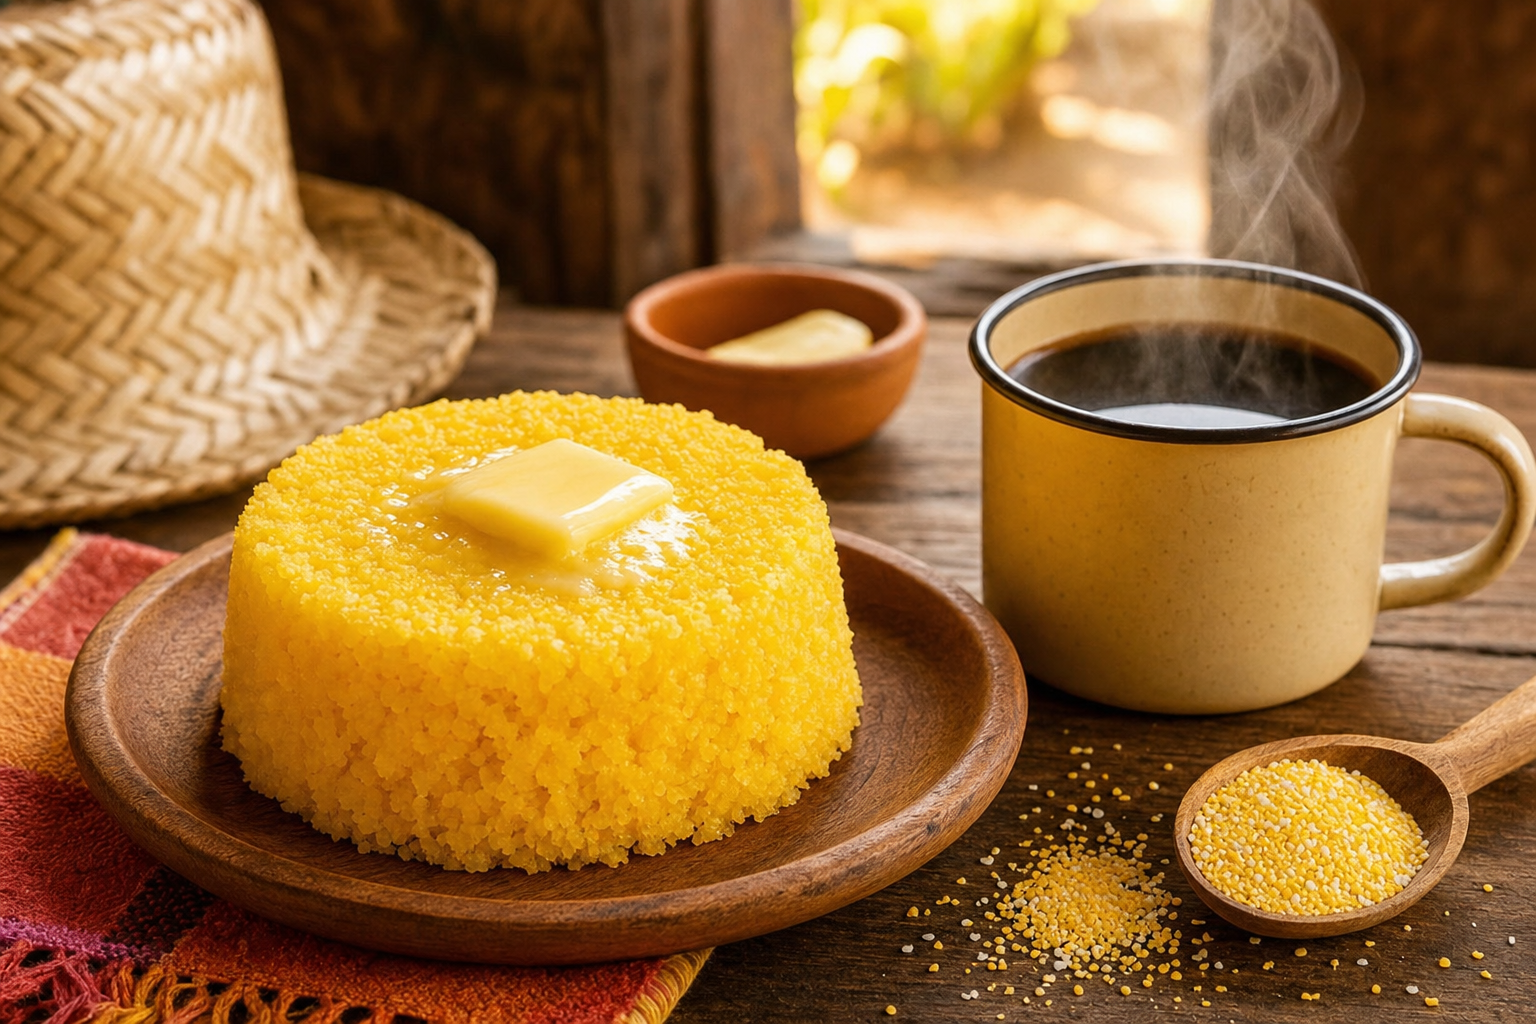
\includegraphics[width=0.85\textwidth]{livro-cuscuz-imagens/cuscuz-nordestino.png}
\caption{O clássico cuscuz nordestino: flocão de milho cozido no vapor, servido com manteiga derretida e café.}
\label{fig:cuscuz-nordestino-cap3}
\end{figure}

\section{História e Origem}

O cuscuz nordestino --- também chamado cuscuz de milho ou, arcaicamente, pão de milho --- é a versão mais emblemática do cuscuz no Brasil. Nascido da adaptação do cuscuz magrebino à realidade brasileira, tornou-se um símbolo de identidade e resistência do povo nordestino.

O poeta pernambucano Ascenso Ferreira registou em poesias publicadas em 1963 que o cuscuz não se restringiu à culinária indígena, mas manteve-se presente durante o período escravocrata, associado à alimentação de negros e mestiços, e comercializado por quituteiras nas ruas e feiras. O Quilombo dos Palmares, em Alagoas, destaca-se como uma das comunidades negras que adotaram a prática indígena de preparo do cuscuz.

Em 2021, o estado de Pernambuco declarou o cuscuz como Património Cultural e Imaterial do estado. Anualmente, a 19 de março, celebra-se o Dia Mundial do Cuscuz.

\section{Ingredientes e Preparo}

O cuscuz nordestino é feito com \textbf{farinha de milho flocada} --- também conhecida como \textbf{flocão} de milho --- que se distingue do fubá por ser mais grossa e granulada. A farinha é humedecida com água e sal até atingir a consistência de areia molhada, e depois cozida no vapor numa \textbf{cuscuzeira}, panela tradicional composta por dois compartimentos: o inferior para a água e o superior para a massa.

O cozimento é rápido --- não mais de 10 minutos --- e o resultado é uma massa fofa, quente e aromática.

\section{Modos de Servir}

O cuscuz nordestino é extremamente versátil. Pode ser servido:

\begin{itemize}
    \item \textbf{Simples}, apenas com manteiga a derreter por cima.
    \item \textbf{Com ovo}, seja cozido, frito ou pochê.
    \item \textbf{Com leite}, vertido sobre o cuscuz quente.
    \item \textbf{Com carne de sol} ou charque desfiada.
    \item \textbf{Com queijo coalho} derretido.
    \item \textbf{Com leite de coco}, versão doce e cremosa.
    \item \textbf{Com calabresa, frango, sardinha}, em versões mais substanciais.
\end{itemize}

É o café da manhã dos campeões no Nordeste, mas também marca presença no almoço e no jantar.

% ============================================================
% CAPÍTULO 4
% ============================================================
\chapter{Cuscuz Paulista: História, Polémica e Sabor}

\begin{figure}[htbp]
\centering
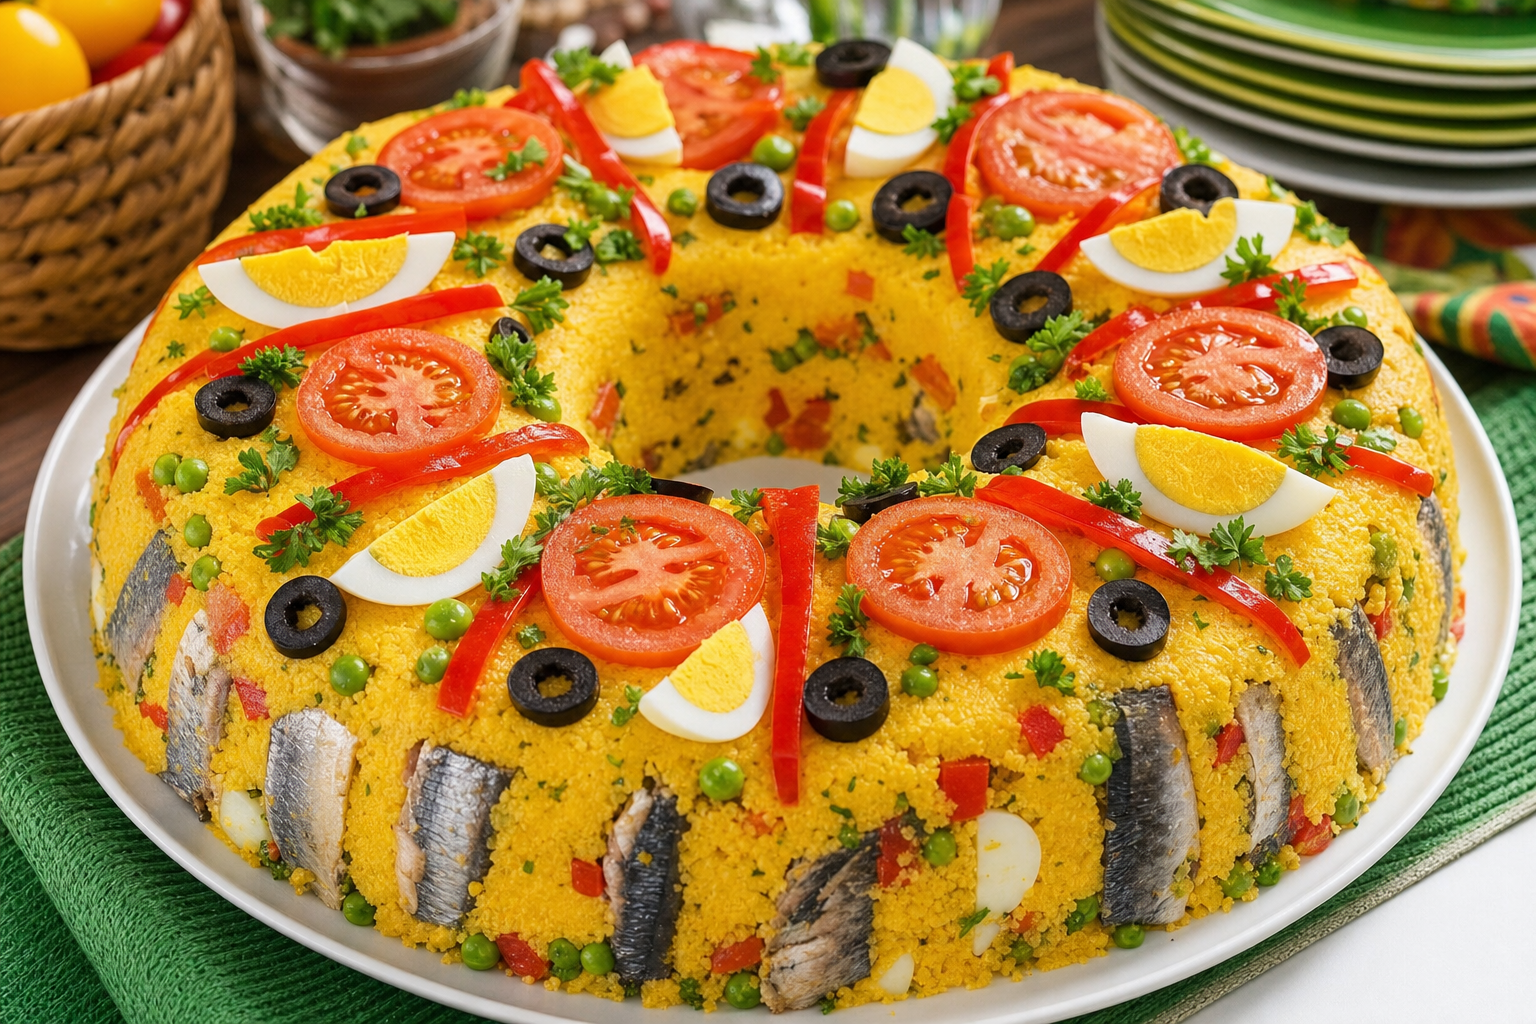
\includegraphics[width=0.85\textwidth]{livro-cuscuz-imagens/cuscuz-paulista.png}
\caption{Cuscuz paulista moldado e decorado com ovos, azeitonas e ervilhas, servido em fatias como um bolo salgado.}
\label{fig:cuscuz-paulista}
\end{figure}

\epigraph{O cuscuz paulista é provavelmente um dos pratos mais polémicos da internet... e um dos mais saborosos das festas brasileiras.}{Adaptado de BBC News Brasil}

\section{Origens Bandeirantes}\label{sec:origens}

O cuscuz paulista tem raízes profundas na história de São Paulo. Entre os séculos XVII e XVIII, os bandeirantes paulistas --- desbravadores que percorriam o interior do Brasil em busca de ouro, indígenas e riquezas --- precisavam de alimentos práticos, nutritivos e que se conservassem bem durante as longas viagens.

Assim nasceu o cuscuz paulista: uma refeição completa, preparada com farinha de milho e todos os ingredientes disponíveis --- carnes, peixes, legumes --- cozidos numa só panela. O naturalista francês Auguste de Saint-Hilaire, que viajou por São Paulo em 1822, registou o cuscuz como um dos pratos típicos das refeições dos paulistas.

\section{O Papel das Quitandeiras}

No século XIX, as quitandeiras --- mulheres negras escravizadas ou forras --- começaram a vender cuscuz pelas ruas de São Paulo em tabuleiros. A receita da época incluía camarões, bagres e piquiras (pequenos peixes de água doce).

O cuscuz de bagre era tão apreciado que chegou a ser servido nos camarotes do antigo Teatro Ópera, no Pátio do Colégio. Uma coluna do \textit{Diário de S. Paulo} de 1868 recorda com nostalgia: \textit{“em que se comia cuscuz de bagre nos camarotes e dizem alguns que até tutu de feijão”}.

As quitandeiras desempenharam um papel fundamental na disseminação do cuscuz paulista, transformando-o de simples farnel de bandeirantes em iguaria urbana. Muitas destas mulheres conseguiram sustentar as suas famílias e até comprar a própria liberdade através da venda de alimentos.

\section{Características e Ingredientes}

Ao contrário do cuscuz nordestino, que é mais simples e soltinho, o cuscuz paulista é um prato \textbf{elaborado, húmido e compacto}, servido em fatias como um bolo salgado.

Os ingredientes típicos incluem:
\begin{itemize}
    \item Farinha de milho amarela (fubá)
    \item Molho de tomate, cebola, alho, pimentão e cheiro-verde
    \item Sardinha, camarão, atum ou frango desfiado
    \item Ovos cozidos
    \item Azeitonas, ervilhas, milho verde e palmito
    \item Sal, temperos e azeite de dendê (em algumas versões)
\end{itemize}

O preparo consiste em refogar todos os ingredientes, misturar com a farinha de milho até formar uma massa compacta, colocar numa forma com furo central (previamente decorada com ovos, azeitonas e ervilhas) e cozinhar no vapor. Depois de frio, desenforma-se como um pudim salgado, revelando uma apresentação colorida e festiva.

\section{Importância Cultural}

O cuscuz paulista é considerado património cultural do estado de São Paulo. É prato obrigatório nas festas juninas, no Natal e no Ano Novo, integrando a ceia de muitas famílias tradicionais ao lado do peru e da rabanada.

Apesar de ser alvo de piadas e polémicas na internet --- sobretudo entre nordestinos e paulistas --- o cuscuz paulista carrega uma história riquíssima de adaptação, criatividade e resistência cultural.

% ============================================================
% CAPÍTULO 5
% ============================================================
\chapter{Cuscuz Marroquino: O Património da Humanidade}

\epigraph{O cuscuz marroquino não é apenas comida; é um gesto de hospitalidade, um símbolo de partilha e união familiar.}{\textit{Culinária Marroquina}}

\begin{figure}[htbp]
\centering
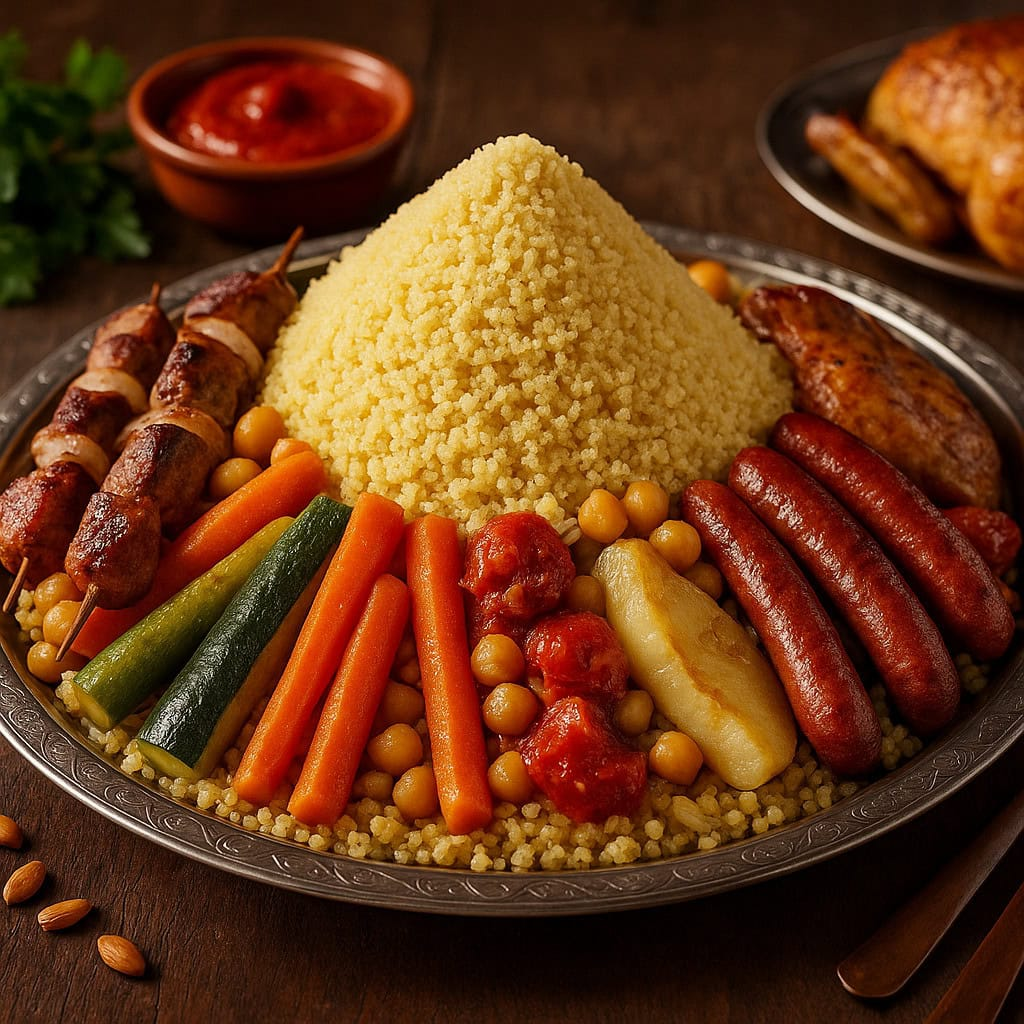
\includegraphics[width=0.85\textwidth]{livro-cuscuz-imagens/cuscuz-marroquino.jpg}
\caption{Cuscuz marroquino servido com carne, legumes e grão-de-bico, típico das refeições em família no Magrebe.}
\label{fig:cuscuz-marroquino-cap5}
\end{figure}

\section{História Milenar}

O cuscuz marroquino --- ou \textit{couscous}, na sua designação francesa --- é o herdeiro direto da tradição berbere. Feito a partir de \textbf{sêmola de trigo durum}, um trigo de grão duro, é a base da cozinha do Magrebe e um dos pratos mais antigos do mundo ainda em preparação quotidiana.

Estima-se que o cuscuz seja consumido há cerca de dois milénios no Norte de África. Os berberes, pastores nómadas, aperfeiçoaram a técnica de enrolar a sêmola com água para formar pequenos grânulos que coziam ao vapor, criando um alimento leve, nutritivo e de fácil conservação.

\section{O Preparo Tradicional}

O cuscuz marroquino tradicional é cozido numa \textbf{cuscuzeira} (\textit{couscoussier} em francês), panela de dois andares onde a parte inferior coze lentamente um ensopado de carne e legumes, e a parte superior recebe o vapor que coze a sêmola.

A sêmola é primeiro humedecida e esfregada entre as mãos para evitar grumos, depois cozida no vapor por cerca de 20 a 30 minutos. O processo pode repetir-se duas ou três vezes, arejando a sêmola com um garfo entre cada cozedura, para obter grãos leves e soltos.

\section{Variações Regionais}

\begin{itemize}
    \item \textbf{Cuscuz de sete vegetais:} a versão marroquina mais clássica, com frango, cenoura, nabo, abóbora, courgette, grão-de-bico e passas, servida às sextas-feiras.
    \item \textbf{Seffa:} versão doce, com mel, amêndoas, canela, flor de laranjeira, passas e manteiga, servida em festas e casamentos, frequentemente polvilhada com açúcar em pó e canela.
    \item \textbf{Cuscuz de borrego:} popular na Tunísia, com carne de borrego e frutas secas como damascos e ameixas.
    \item \textbf{Cuscuz de peixe:} comum nas zonas costeiras, com peixe fresco, legumes e molho picante.
    \item \textbf{Maftoul:} versão palestiniana, feita com triguilho rolado à mão com farinha de trigo, servido com frango e grão-de-bico.
\end{itemize}

\section{Reconhecimento Mundial}

Em 2020, o cuscuz --- os conhecimentos e práticas relacionadas à sua preparação --- foi inscrito pela UNESCO na Lista Representativa do Património Cultural Imaterial da Humanidade. A candidatura, submetida conjuntamente por Marrocos, Argélia, Tunísia e Mauritânia, reconheceu o papel central do cuscuz na identidade cultural, na coesão social e na hospitalidade dos povos do Magrebe.

Em França, o cuscuz foi eleito o terceiro prato mais popular do país em 2011, demonstrando a sua enorme capacidade de atravessar fronteiras e conquistar paladares.

% ============================================================
% CAPÍTULO 6
% ============================================================
\chapter{Cuscuz de Tapioca: A Sobremesa que Veio da Cozinha das Escravas}

\begin{figure}[htbp]
\centering
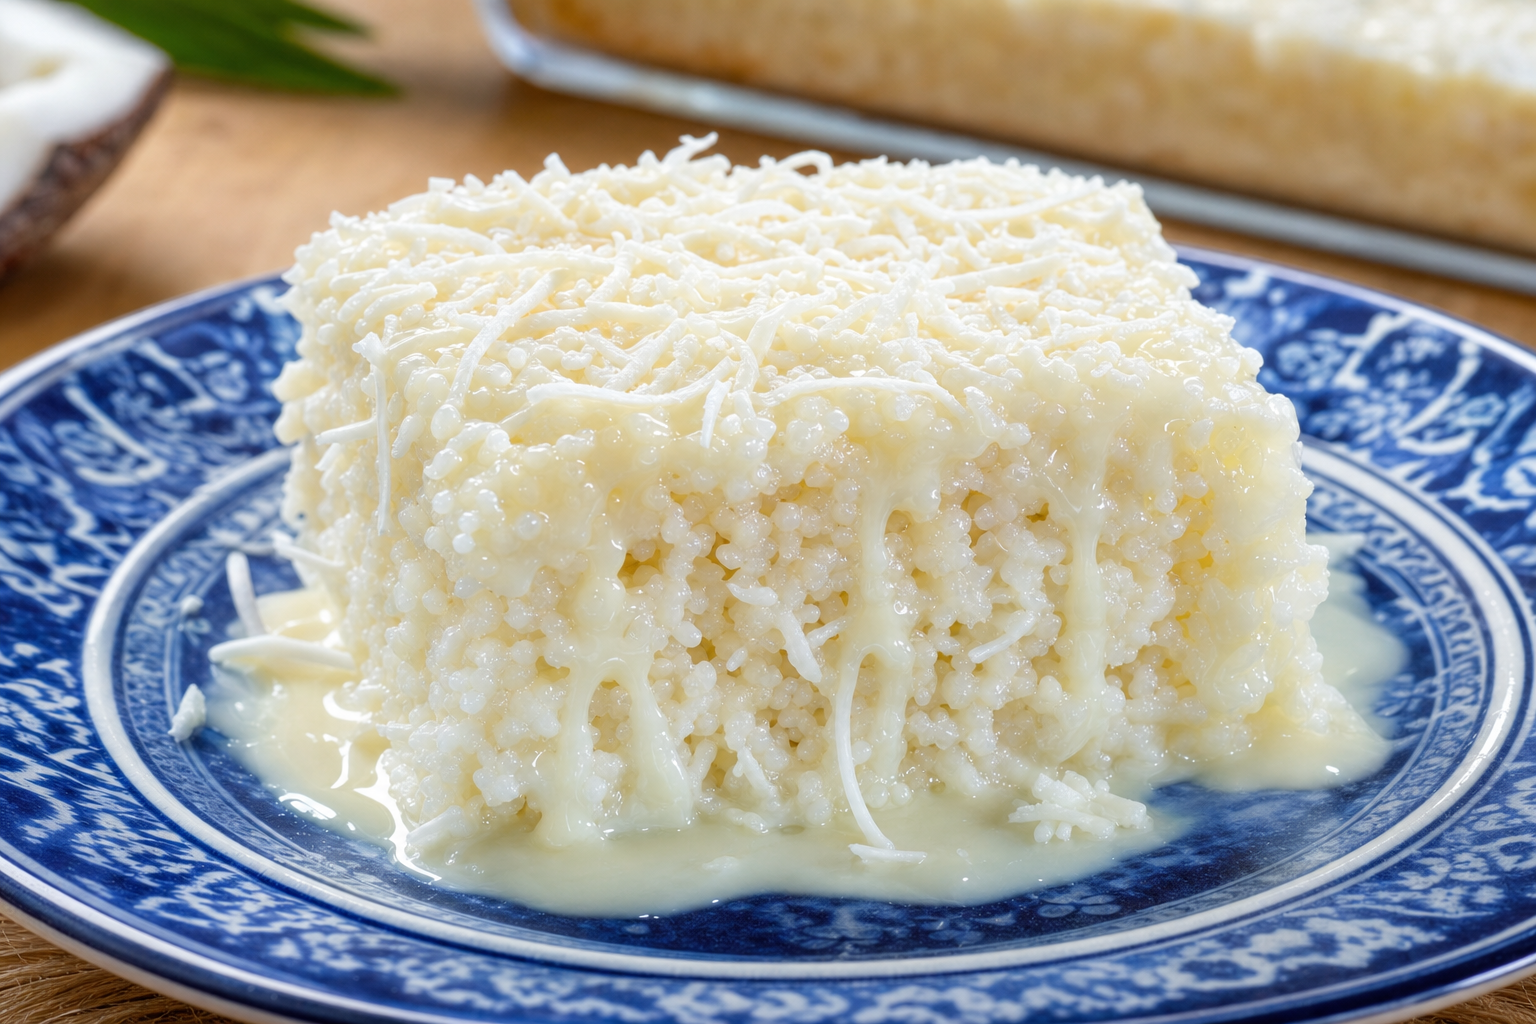
\includegraphics[width=0.85\textwidth]{livro-cuscuz-imagens/cuscuz-tapioca.png}
\caption{Cuscuz de tapioca doce, sobremesa cremosa com coco e leite de coco, típica da culinária brasileira.}
\label{fig:cuscuz-tapioca}
\end{figure}

\epigraph{Nas mãos das africanas escravizadas, a tapioca indígena encontrou açúcar e leite, e nasceu o cuscuz doce.}{Culinária Brasileira}

\section{Origem Baiana}

O cuscuz de tapioca --- também conhecido como cuscuz branco, cuscuz carioca ou pudim de tapioca --- é um doce tipicamente brasileiro, de origem baiana. Distingue-se dos outros cuscuz por ser feito a partir da fécula extraída da mandioca, a tapioca, ingrediente de origem indígena.

Acredita-se que o cuscuz de tapioca foi criado por mulheres africanas escravizadas que trabalhavam nas cozinhas das casas-grandes e dos conventos. Elas tinham acesso a ingredientes indígenas como a mandioca e a tapioca, mas também a ingredientes europeus como o açúcar e o leite. Combinando tudo, criaram esta sobremesa delicada e refrescante.

\section{Características e Preparo}

Ao contrário dos cuscuz salgados, o cuscuz de tapioca é uma sobremesa cremosa e gelada. A tapioca granulada é hidratada em leite de coco e leite comum, adoçada com açúcar e cozida até formar um mingau espesso. Depois de fria, a massa é colocada numa forma e refrigerada, adquirindo consistência de pudim.

Os ingredientes básicos são:
\begin{itemize}
    \item Tapioca granulada (também chamada de sagu de tapioca)
    \item Leite de coco
    \item Leite integral
    \item Açúcar
    \item Coco ralado
    \item Leite condensado (em muitas versões modernas)
\end{itemize}

Pode ser servida simples ou acompanhada por calda de ameixa, frutas vermelhas ou leite condensado. É uma sobremesa refrescante, especialmente popular no Sudeste do Brasil.

\section{O Cuscuz de Tapioca Salgado}

Embora a versão doce seja a mais conhecida, existe também o cuscuz de tapioca salgado, preparado com os mesmos princípios mas com sal e temperos salgados no lugar do açúcar e do coco, muitas vezes acompanhado de carne seca ou camarão.

% ============================================================
% CAPÍTULO 7
% ============================================================
\chapter{Outras Variações Regionais no Brasil}

\section{Cuscuz Campeiro (Rio Grande do Sul)}

No sul do Brasil, o cuscuz gaúcho --- ou cuscuz campeiro --- é uma versão robusta que reflete a tradição pecuária da região. Leva charque (carne seca), carne de gado, linguiça, farinha de milho e temperos. É uma refeição completa, consumida frequentemente no ambiente rural dos pampas.

\section{Cuscuz Mineiro}

Em Minas Gerais, o cuscuz apresenta duas versões distintas registadas por Maria Stella Libânio Christo no livro \textit{Fogão de Lenha}:
\begin{itemize}
    \item \textbf{Cuscuz de fubá mimoso:} cozido no vapor em cuscuzeira untada com manteiga, simples e delicioso.
    \item \textbf{Cuscuz torrado:} feito com farinha de trigo e fubá mimoso misturados com banha de porco derretida, assado no forno --- uma textura e sabor únicos.
\end{itemize}

\section{Bijajica (Santa Catarina)}

O bijajica é o cuscuz açoriano-catarinense, feito à base de mandioca, amendoim cru e açúcar mascavo, cozido no vapor da cuscuzeira. Reflete a forte influência da culinária açoriana no litoral catarinense.

\section{Mandipuva (Paraná)}

No Paraná, a mandipuva é um cuscuz feito com mandioca fermentada e espremida, temperada com sal, erva-doce e canela, ou acrescida de amendoim, ovos e banha de porco.

\section{Cuscuz de Inhame (Bahia)}

Na Bahia, há variações que utilizam inhame e farinha de mandioca, combinando ingredientes africanos e indígenas numa fusão saborosa.

\section{Cuscuz de Arroz e Tapioca (Maranhão)}

No Maranhão, o cuscuz é preparado com flocos de arroz e tapioca, criando uma textura única que reflete a diversidade de cereais disponíveis na região.

% ============================================================
% CAPÍTULO 8
% ============================================================
\chapter{O Cuscuz pelo Mundo}

\section{Cabo Verde}

Em Cabo Verde, o cuscuz é um bolo tradicional feito com farinha de milho, cozido a vapor num recipiente de barro especial chamado \textit{binde}, análogo à cuscuzeira. Leva pouco açúcar e é normalmente comido quente, às fatias, com manteiga ou mel de cana.

\section{Sicília e Sul da Itália}

Na Sicília, o cuscuz (\textit{cuscus}) é um prato tradicional da cidade de Trapani, herança da dominação árabe na ilha. O \textit{cuscus alla trapanese} é feito com sêmola e servido com um caldo de peixe, criando uma fusão única entre a tradição norte-africana e os ingredientes do Mediterrâneo.

\section{Israel e Mundo Judeu}

O \textit{ptitim} israelita --- também conhecido como \textit{couscous israelita} --- é uma variação de pasta de trigo tostada, com grãos maiores e textura mais mastigável que o cuscuz marroquino. Foi criado na década de 1950 como substituto do arroz durante um período de racionamento.

\section{França}

Em França, o cuscuz foi amplamente adoptado durante o período colonial e tornou-se um dos pratos mais populares do país. O \textit{plat couscous} típico francês consiste em sêmola de cuscuz servida com ensopado de carne, legumes e caldo picante, frequentemente acompanhado de harissa.

% ============================================================
% RECEITAS
% ============================================================
\chapter{Receitas}

\section{Receita de Cuscuz Nordestino}

\textbf{Ingredientes:}
\begin{itemize}
    \item 2 xícaras de flocão de milho
    \item 1 colher de chá de sal
    \item Água para humedecer (aproximadamente 1 xícara)
\end{itemize}

\textbf{Modo de preparo:}
\begin{enumerate}
    \item Numa tigela grande, misture o flocão com o sal.
    \item Adicione água aos poucos, misturando com as mãos até a farinha ficar com textura de areia molhada --- nem seca nem empapada.
    \item Deixe descansar por 10 minutos para hidratar.
    \item Coloque a massa na cuscuzeira (parte superior) sem apertar, apenas nivelando.
    \item Leve ao fogo médio com água na parte inferior da cuscuzeira e cozinhe por 10 minutos após a água ferver.
    \item O cuscuz está pronto quando a massa estiver macia e soltinha.
\end{enumerate}

\textit{Sugestão: sirva com manteiga, ovo cozido ou carne de sol desfiada.}

\section{Receita de Cuscuz Paulista}

\textbf{Ingredientes:}
\begin{itemize}
    \item 2 xícaras de farinha de milho (fubá)
    \item 1 xícara de molho de tomate
    \item 1 cebola picada
    \item 2 dentes de alho picados
    \item 1 pimentão verde picado
    \item 1 tomate picado
    \item 1 lata de sardinha (ou 200g de frango desfiado)
    \item 2 ovos cozidos em rodelas
    \item 1/2 xícara de azeitonas
    \item 1/2 xícara de ervilhas
    \item 1/2 xícara de milho verde
    \item 1 vidro de palmito picado
    \item Cheiro-verde, sal e azeite a gosto
\end{itemize}

\textbf{Modo de preparo:}
\begin{enumerate}
    \item Refogue a cebola, o alho e o pimentão no azeite.
    \item Junte o tomate, o molho de tomate e deixe apurar.
    \item Adicione a sardinha ou frango, azeitona, palmito, ervilha e milho.
    \item Tempere com sal e cheiro-verde.
    \item Acrescente a farinha de milho aos poucos, mexendo sempre, até obter uma massa húmida e compacta.
    \item Unte uma forma de furo central com azeite e decore o fundo com rodelas de ovo, azeitonas e ervilhas.
    \item Coloque a massa na forma, apertando ligeiramente.
    \item Leve ao vapor por 15-20 minutos.
    \item Deixe esfriar, desenforme e sirva em fatias.
\end{enumerate}

\section{Receita de Cuscuz Marroquino}

\textbf{Ingredientes:}
\begin{itemize}
    \item 2 xícaras de sêmola de trigo para cuscuz
    \item 2 xícaras de água
    \item 1 colher de chá de sal
    \item 2 colheres de sopa de azeite
    \item 500g de frango ou carneiro
    \item 1 cebola
    \item 3 cenouras
    \item 2 nabos
    \item 1 abobrinha
    \item 1/2 xícara de grão-de-bico cozido
    \item 1 colher de chá de cúrcuma, canela e gengibre
    \item Salsa e coentros picados
\end{itemize}

\textbf{Modo de preparo:}
\begin{enumerate}
    \item Tempere a carne com sal e especiarias e refogue com cebola no azeite.
    \item Adicione água e cozinhe em lume brando por 30 minutos.
    \item Junte os legumes cortados e o grão-de-bico e cozinhe até macios.
    \item Noutra panela, humedeça a sêmola com um fio de água e esfregue entre as mãos.
    \item Coloque a sêmola na cuscuzeira e cozinhe no vapor do caldo por 20 minutos.
    \item Retire, areie com um garfo, repita a cozedura por mais 10 minutos.
    \item Sirva a sêmola numa travessa, regue com o caldo e cubra com a carne e os legumes.
\end{enumerate}

\section{Receita de Cuscuz de Tapioca (Doce)}

\textbf{Ingredientes:}
\begin{itemize}
    \item 1 xícara de tapioca granulada
    \item 1 xícara de leite de coco
    \item 2 xícaras de leite
    \item 1/2 xícara de açúcar
    \item 1/2 xícara de coco ralado
    \item 1 pitada de sal
    \item 1 lata de leite condensado (opcional)
\end{itemize}

\textbf{Modo de preparo:}
\begin{enumerate}
    \item Numa tigela, misture a tapioca com o leite de coco e o leite. Deixe hidratar por 30 minutos.
    \item Leve ao lume médio com o açúcar, o coco ralado e o sal, mexendo sempre até engrossar.
    \item Cozinhe por mais 5 minutos em lume baixo.
    \item Coloque numa forma de pudim humedecida e deixe arrefecer.
    \item Leve ao frigorífico por no mínimo 4 horas.
    \item Desenforme e sirva frio, com leite condensado ou calda de frutas vermelhas.
\end{enumerate}

\section{Receita de Cuscuz de Tapioca Salgado}

\textbf{Ingredientes:}
\begin{itemize}
    \item 1 xícara de tapioca granulada
    \item 2 xícaras de leite
    \item 1 colher de chá de sal
    \item 2 colheres de sopa de manteiga
    \item 200g de carne seca dessalgada e desfiada
    \item 1 cebola picada
    \item Cheiro-verde a gosto
\end{itemize}

\textbf{Modo de preparo:}
\begin{enumerate}
    \item Refogue a carne seca com a cebola na manteiga.
    \item Hidrate a tapioca no leite com sal por 30 minutos.
    \item Leve ao lume médio mexendo até engrossar.
    \item Misture a carne seca refogada e o cheiro-verde.
    \item Coloque na forma, deixe esfriar e desenforme.
\end{enumerate}

% ===========================================================%
% CONCLUSÃO
% ===========================================================%
\chapter*{Conclusão}
\addcontentsline{toc}{chapter}{Conclusão}

O cuscuz é, acima de tudo, uma história de adaptação e criatividade. Das mãos dos pastores berberes no Norte de África às cozinheiras nordestinas, das quitandeiras paulistas às avós que fazem cuscuz de tapioca, cada versão conta a história de um povo, de uma região e de uma forma de transformar simples grãos em alimento que aquece o corpo e a alma.

Seja no café da manhã com manteiga, na festa junina com sardinha, no jantar de sexta-feira com legumes, ou na sobremesa gelada de coco, o cuscuz une continentes, tempos e sabores numa só travessa.

Que este livro ajude a preservar e celebrar esta herança tão rica --- e que nunca faltem cuscuz na sua mesa.

% ============================================================
% REFERÊNCIAS
% ============================================================
\chapter*{Referências}
\addcontentsline{toc}{chapter}{Referências}

\begin{enumerate}
    \item WIKIPÉDIA. \textit{Cuscuz}. Disponível em: \url{https://pt.wikipedia.org/wiki/Cuscuz}
    \item WIKIPÉDIA. \textit{Cuscuz nordestino}. Disponível em: \url{https://pt.wikipedia.org/wiki/Cuscuz_nordestino}
    \item WIKIPÉDIA. \textit{Cuscuz paulista}. Disponível em: \url{https://pt.wikipedia.org/wiki/Cuscuz_paulista}
    \item WIKIPÉDIA. \textit{Cuscuz de tapioca}. Disponível em: \url{https://pt.wikipedia.org/wiki/Cuscuz_de_tapioca}
    \item CÂMARA CASCUDO, Luís da. \textit{História da Alimentação no Brasil}. Global Editora, 2004.
    \item FOLHA DE S.PAULO. \textit{Tipos de cuscuz}. Web Stories, 2021.
    \item GLOBO RECEITAS. \textit{Cuscuz nordestino, marroquino, paulista e doce: entenda a diferença}. 2021.
    \item UOL. \textit{Cuscuz não é só o paulista: varie o menu com 5 receitas doces e salgadas}.
    \item INSTITUTO GOURMET. \textit{Como é o cuscuz em cada região do Brasil}.
    \item IDEAC - Instituto de Defesa de Consumidores. \textit{Cuscuz: símbolo afetivo do Nordeste e de todo o Brasil}. 2024.
    \item COMES. \textit{O som da cuscuzeira: a história do cuscuz no Brasil}. 2019.
    \item BBC NEWS BRASIL. \textit{Cuscuz paulista: por que prato 'odiado' na internet é importante na história da culinária brasileira}. 2024.
    \item UNESCO. \textit{Couscous: knowledge, skills and practices}. Inscrito em 2020 na Lista Representativa do Património Cultural Imaterial da Humanidade.
\end{enumerate}

\end{document}
